React es una biblioteca de JavaScript declarativa, eficiente y flexible creada en 2013 por el equipo de desarrollo de Facebook. React quería que las interfaces de usuario fueran más modulares (o reutilizables) y más fáciles de mantener. Según el sitio web de React, se utiliza para \textit{construir componentes encapsulados que administran su propio estado, y unirlos para crear interfaces de usuario complejas}. React es una biblioteca JavaScript que permite componer interfaces de usuario complejas a partir de piezas de código pequeñas y aisladas llamadas \textit{componentes}.
\vspace{0.8cm}

En términos generales, al crear aplicaciones con ReactJS, se crean componentes que corresponden a distintos elementos de una interfaz de usuario. Después se organizan estos elementos dentro de componentes de orden superior que definen la estructura de la aplicación. Es importante destacar que cada componente en una aplicación React se rige por principios estrictos de gestión de datos. Interfaces avanzadas comúnmente involucran datos complejos y manejo de estado. ReactJS es limitado y tiene como objetivo darnos las herramientas para poder anticipar cómo se verá una aplicación con un conjunto de circunstancias dado.

\subsection{Componentes React}
Un componente es una pequeña parte de la interfaz de usuario. Todas las piezas reutilizables de una página web se abstraen en estos elementos. Son similares, en conceptos, a cosas como \glspl{widget} y módulos. React se define a sí mismo como una biblioteca para construir interfaces de usuario. Como tal, cuando se piensa en una interfaz de usuario, se debe pensar en ella en términos de los componentes más pequeños posibles que se puedan definir. La razón por la que existe este paradigma es para disminuir el acoplamiento (cuánto dependen los unos de los otros) y aumentar la cohesión (qué tan bien funcionan juntas las diferentes cosas).
\vspace{0.8cm}

Cada uno de estos fragmentos es un bloque de código independiente y reutilizable, que divide la interfaz de usuario en partes más pequeñas. Incluyen código que define cómo se crean los elementos en el \acrshort{dom} y cómo los usuarios pueden interactuar con ellos. Los componentes se pueden definir únicamente en JavaScript o se pueden definir en un superconjunto (o variación extendida) de JavaScript llamado JSX, que se explica en temas posteriores.
\vspace{0.8cm}

\begin{figure}[H]
  \centering
  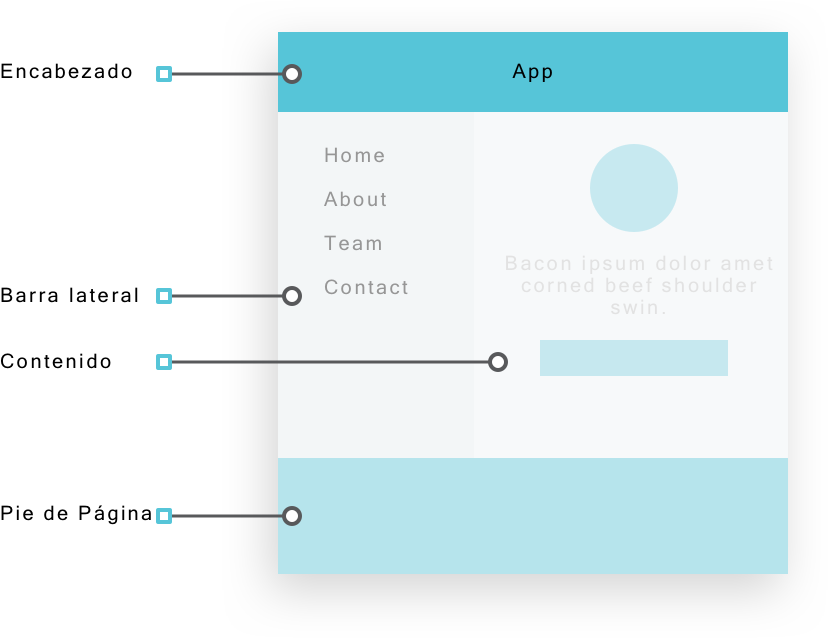
\includegraphics[width=0.8\textwidth]{components}
  \caption{Componentes principales de una página web. (Fuente: Elaboración propia)}
\end{figure}
En primer lugar, hay un elemento principal llamado componente APP. Este componente de la aplicación contiene cuatro fragmentos secundarios o se divide en cuatro componentes:
\begin{enumerate}
  \item Encabezado
  \item Barra lateral
  \item Contenido
  \item Pie de página
\end{enumerate}
La función de cada componente se manejará independientemente con otros componentes. Cada componente es una pieza reutilizable, y se puede pensar en cada componente de forma aislada.
\vspace{0.8cm}

Dentro de un componente, tendremos subcomponentes o componentes dentro de un componente padre. Esos serán reutilizables también. En pocas palabras, un componente es una clase o función de JavaScript que opcionalmente acepta entradas, es decir, propiedades (props) y devuelve un elemento que describe cómo debería lucir una sección de la interfaz de usuario.
\vspace{0.8cm}

\lstinputlisting[style=ES6, caption=Ejemplo de página con componentes ReactJS]{code/react-example.js}

\subsection{DOM Virtual}
En el desarrollo web de software, \acrshort{dom} significa Modelo de Objeto de Documento (Document Object Model) y representa la estructura de los elementos en una página web. El HTML DOM se construye como un árbol de objetos.

Algunas bibliotecas de JavaScript, como jQuery, manipulan los elementos DOM directamente, cambiando sus atributos, agregando o eliminando componentes. Sin embargo, en lugar de cambiar el DOM directamente, React usa un DOM virtual, que es una replicación virtual del árbol DOM actual. En consecuencia, React puede manipular el DOM virtual innumerables veces y comparar su estado con el DOM real. De esta manera, React sabe exactamente qué elemento cambió y luego actualiza solo ese elemento específico en la pantalla.

Detrás de escena, React hace un gran trabajo para editar y volver a \gls{renderizar} eficientemente el DOM cuando algo en la interfaz necesita cambiar. Este enfoque le brinda al desarrollador una gran flexibilidad y sorprendentes ganancias de rendimiento porque ReactJS calcula con anticipación qué cambios se deben realizar en el DOM y actualiza los árboles DOM en consecuencia. De esta manera, ReactJS evita las costosas operaciones DOM y realiza actualizaciones de manera eficiente \cite{stefanov}.